\documentclass[AnalisiDeiRequisiti.tex]{subfiles}

\begin{document}

\chapter{Casi d'uso}
\section{Attori dei casi d'uso}
\subsection{Attori primari}
\begin{enumerate}
	\begin{figure}[h]
		\centering
		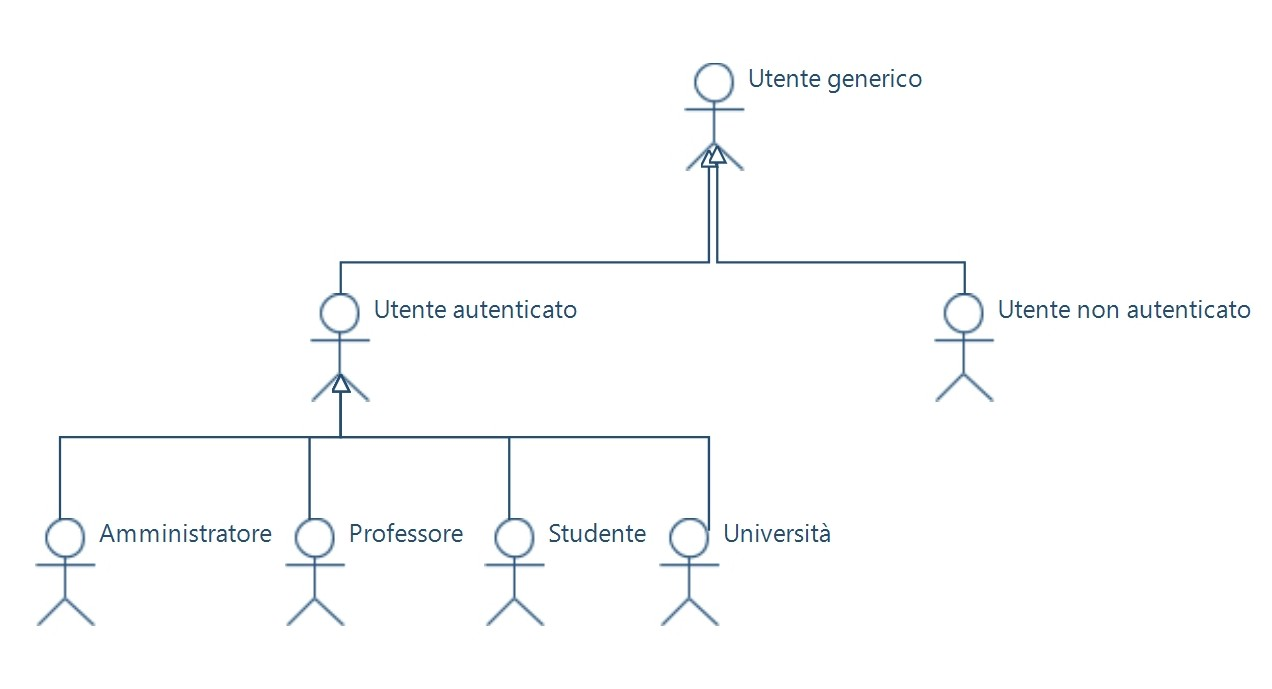
\includegraphics[width=0.6\linewidth]{attoriPrincipali.jpg}
		\caption{Gerarchia attori primari}
		\label{fig:attoriprincipali}
	\end{figure}
	
	\item \textbf{Utente generico}\\
	Si riferisce ad un utente generico che accede al sito\\
	
	\item \textbf{Utente non autenticato}\\
	Ci si riferisce ad un utente generico con non ha ancora effettuato il login.\\
	
	\item \textbf{Utente autenticato}\\
	 Ci si riferisce ad un utente generico con chiave valida ed autenticato nel sistema tramite la procedura di login.\\
	
	\item \textbf{Amministratore}\\
	Ci si riferisce ad un utente autenticato nel sistema nel ruolo di amministratore\\
	
	\item \textbf{Professore}\\
	Ci si riferisce ad un utente autenticato nel sistema nel ruolo di professore.\\
	
	\item \textbf{Studente}\\
	Ci si riferisce ad un utente autenticato nel sistema nel ruolo di studente\\	
\end{enumerate}

\subsection{Attori secondari}
\begin{enumerate}
	\item \textbf{MetaMask}\\
	Plugin del browser MetaMask per interfacciarsi ad una rete Ethereum.\\
	
	\item \textbf{Ufficio immatricolazioni universitario}\\
	Entità fisica che consente l'immatricolazione.\\
\end{enumerate}

\section{Elenco dei casi d'uso}

%TODO controllare posizione immagine
\begin{figure}[h]
	\centering
	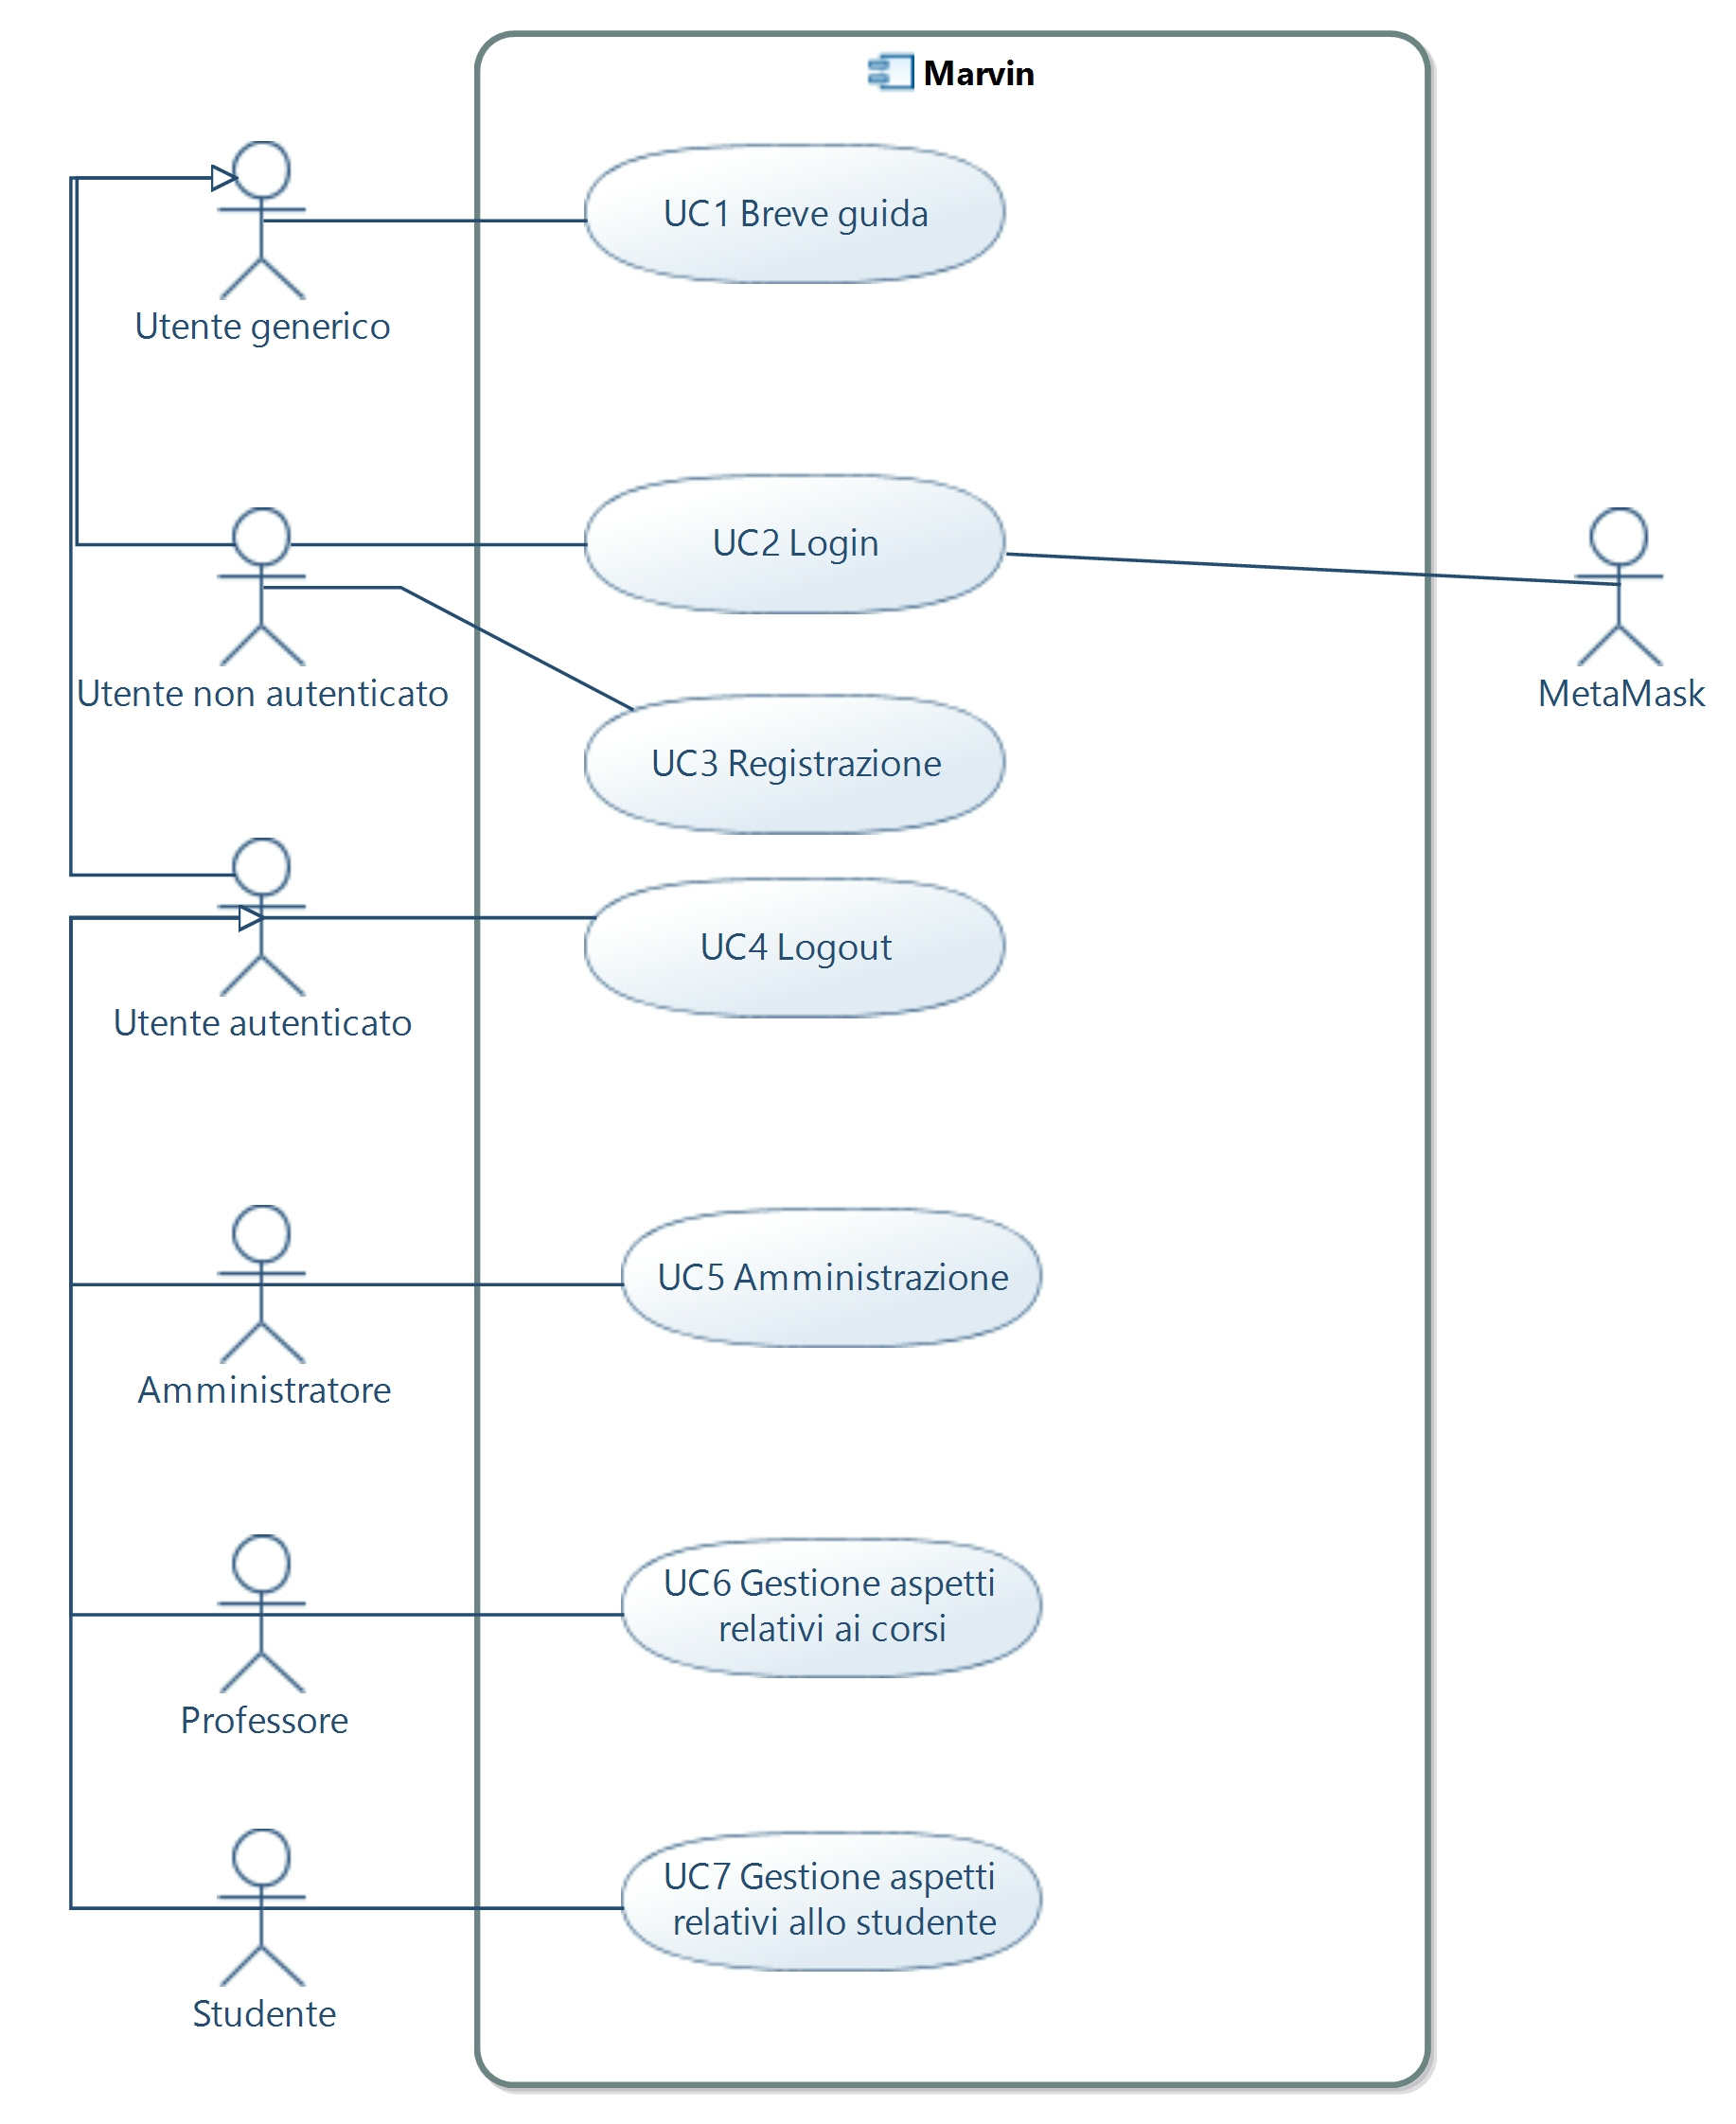
\includegraphics[width=0.6\linewidth]{UC.jpg}
	\caption{Casi d'uso basilari}
	\label{fig:UC}
\end{figure}

%   -------------------------------------------------------------------------------------
%   ----------                 MODELLO PER GLI USER CASE              -------------------
%   -------------------------------------------------------------------------------------
\begin{comment}
\subsection{UCX - Nome}
\begin{itemize}
	\item \textbf{Attori primari:} ;\\
	\item \textbf{Attori secondari:} ;\\
	\item \textbf{Scopo e descrizione:} ;\\
	\item \textbf{Scenario principale:} ;\\
	\item \textbf{Scenario alternativo:} ;\\
	\item \textbf{Flusso principale degli eventi:}\\
	\begin{enumerate}
		\item L'utente... ;
		\item L'utente... ;
	\end{enumerate}
	\item \textbf{Estensioni:}\\
	\begin{enumerate}
		\item Se l'utente... ;[UCX.X.X]
	\end{enumerate}
	\item \textbf{Precondizione:} ;\\
	\item \textbf{Postcondizione:} .\\
\end{itemize}
\end{comment}
%
\subsection{UC1 - Breve guida}
\begin{itemize}
	\item \textbf{Attori primari:} Utente generico;\\
	\item \textbf{Scopo e descrizione:} L'utente visualizza una breve guida di introduzione su come installare il plugin MetaMask e su come gestire le chiavi in modo da istruirlo sulle modalità di accesso al sistema;\\
	\item \textbf{Scenario principale:} L'utente accede alla guida;\\
	\item \textbf{Precondizione:} Il sistema è raggiungibile e funzionante e l'utente desidera aprire la guida;\\
	\item \textbf{Postcondizione:} L'utente ha avuto delle nozioni riguardanti l'accesso al sistema.\\
\end{itemize}
\subsection{UC1.1}
\subsection{UC1.2}
\subsection{UC1.2.1}
\subsection{UC2}

\end{document}